\section{Embedding expert knowledge (v2)}\label{sec:expert_v2}
The architecture of the method was completely revised for the second study to ensure the possibility of validating and studying two particular aspects that are of interest:

\begin{itemize}
    \item Generalization improvements by aided learning (expert knowledge).
    \item The specific path loss prediction improvements by the introduction of images.
\end{itemize}

Obtaining generalization in any \gls{ml}-type solutions remains the primary objective of any engineered \gls{ml} solution. Recently, papers introducing model-aided learning have gained popularity due to the achieved generalization properties and the overall simplification in the learning process. It is argued that scientists over the recent decades have constructed quite good models for the reality we live in, and such models should be utilized in \gls{ml} processes. 

What sparked the idea and interest was the work detailed in \cite{Zheng2016}, where a robot is tasked with throwing and catching objects. To throw and catch objects accurately, a predictive model is necessary. The authors show that by utilizing a basic ballistic model for predicting the trajectory in combination with a \gls{ml} system, significant performance gains can be achieved. More specifically, considerable accuracy improvements could be gained by introducing a simple model into the learning process. Even though the model is not accurate, it assisted the learning process to learn the unknown factors associated with the overall throwing system, for instance, the complexity added by the friction of the mechanical joints in the robot etc. This approach reduced the whole learning task from learning the entirety of the system, including the ballistic model, to only learn a correction of the theoretical ballistic model.

Aiding the \gls{ml} models with expert knowledge have been shown to be useful for path loss estimation in \cite{Cavalcanti2017} while expert knowledge for utilization in wireless systems has been hailed as a necessity for future \gls{ml}-based and \gls{dl}-based solutions \cite{Zappone2019}.

Given the recent results of \cite{Thrane2019ComparisonGHz} also seen in section \ref{sec:comparison_ghz_paper}, simple empirical path loss models were evaluated to be valuable. The second version was thus the integration of simple empirical models into the path loss prediction to improve the shortcomings identified in \emph{version 1}. 

\begin{figure*}
    \centering
    \includegraphics{chapters/part_pathloss/model_aided_paper/version2_approach_figure.pdf}
    \caption{The improved approach introduces expert knowledge for improving training stability and testing accuracy.}
    \label{fig:my_label}
\end{figure*}

\subsection{Model architecture}
The model definition was changed and simplified to adjust to isolated experiments. The previous model architecture provided several output metrics of signal quality, in order to determine the performance increase of the model approach this was isolated to a single output parameter, namely \gls{rsrp}. I.e. we define the model as:

\begin{equation}\label{eq:model}
    y(x_n, \mathbf{w}, \bm{\theta}) = \underbrace{z([x_n, L(d)], \mathbf{w}, \bm{\theta})}_{Correction} + L(d)
\end{equation}

Where $z(\cdot)$ is the model of the \gls{dnn}. The $L(d)$ term is an integrated path loss model and provides an estimated link budget. The link budget is estimated as:

\begin{equation}\label{eq:path_loss_model_linkbudget}
L(d) = PL(d) + G_{tx} + L
\end{equation}

Where $PL(d)$ is the \uma{A} path loss model as detailed in Chapter \ref{ch:channelmodellingbasics}. $G_{tx}$ is the estimated transmission power and related gains (constant). We define $L$ as additional losses, such as cable loss and antenna attenuation (constant). 

The defined model is still formalized concerning regression, e.g. Eq. (\ref{eq:dl_model_satellite}) is still the case, however $t_n = RSRP$ and not a vector including such output metrics of \gls{rsrq} etc. The path loss model is integrated into the supervised learning process, as shown in Fig. \ref{fig:combined_model_approach}. The task of the \gls{dnn} is no longer to learn and approximate the received power by itself, it is aided by expert knowledge: a simplified path loss model. We term the output of the \gls{dnn} a \emph{correction}.


\begin{figure}
    \centering
    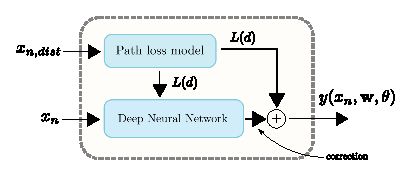
\includegraphics[width=\textwidth]{chapters/part_pathloss/model_aided_paper/combined_model_approach.eps}
    \caption{Combining a path loss model and a \gls{dnn} for estimating \gls{rsrp}.}
    \label{fig:combined_model_approach}
\end{figure}

 $x_{n,dist}$ defines the 3D distance for each measurement point, which, is provided as a feature to the \gls{dnn}. The list of features is the same as presented in Eq. (\ref{eq:dnn_inputs}) with one exception. The estimated link budget is added to the list and is further visualized in Fig. \ref{fig:satellite_model_setup_v2}.
 
The \gls{dnn}, as seen in Fig. \ref{fig:satellite_model_setup_v2} utilize two fully-connected neural networks, and a convolutional neural network. The \gls{nn} termed \texttt{NN} is tasked with managing the engineered features, while the \gls{cnn} is tasked with processing the satellite images. The output of both \gls{nn} are added and combined into a \gls{nn} termed \texttt{NN2}, tasked with processing the information provided by the engineered features and the satellite images resulting in a single output metric. The size of the layers can be seen in Table \ref{tab:cnn_structure} and \ref{tab:nn_structure}.

\begin{figure}
    \centering
    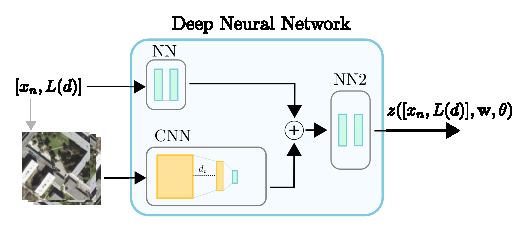
\includegraphics{chapters/part_pathloss/model_aided_paper/setup_model.eps}
    \caption{The Deep Neural Network consists of a convolutional neural network (\emph{CNN}) and two fully connected neural networks, \emph{NN} and \emph{NN2}.}
    \label{fig:satellite_model_setup_v2}
\end{figure}

\subsection{Training}\label{sec:training_v2}
The training of the model was accomplished using Pytorch \cite{Paszke2017AutomaticPyTorch}. The training makes use of backpropagation and the minimization of \gls{mse} loss as described in chapter \ref{ch:mlbasics}. Additionally, the findings of \emph{system v1} highlight the requirement for further generalization techniques. Data augmentation of the images is a common practice to improve dataset size and reduce overfitting during training \cite{Shorten2019ALearning}. The purpose is to feed the algorithm slightly different versions of the same image as to explore the generalization of the method. This was achieved by using a \emph{random  affine  transformation} that shears and rotate the image random but keeps the center of the image invariant. Examples of the data augmentation can be seen in Fig. \ref{fig:data_augmentation}. The transformation utilizes a random rotation angle of $\pm 20$ degrees with $\pm 10$ degrees of shear. The augmentation if applied to the original images for every observation, e.g. for every training iteration. In other words, the original images supplied are randomly transformed during each training iteration. A large finite number of versions of the original image are produced, effectively increasing the amount of available images. Unlike \emph{v1}, grey-scaled images were used to improve generalization. 


\begin{figure}
    \centering
    \includegraphics{chapters/part_pathloss/model_aided_paper/data_augmentation.png}
    \caption{A random affine transformation of satellite images used for data augmentation.}
    \label{fig:data_augmentation}
\end{figure}

A significant number of experiments were completed for scanning hyper-parameters. A complete list of hyper-parameters can be found in Table \ref{tab:cnn_structure}, \ref{tab:nn_structure} and \ref{tab:hyperparam_rest}. A total of $177$ experiments were conducted using different image strategies; the specific number of experiments can be observed in Table \ref{tab:experiments}. The scanning was done with a random search technique, meaning the hyper-parameters were sampled using a uniform distribution between ranges of interest \cite{Bergstra2012RandomOptimization}. A learning rate scheduler was applied with a patience parameter of $5$ epochs and has been shown to improve the convergence of \glspl{nn} \cite{SmithSuper-Convergence:Rates}. The training is terminated when the learning rate reaches a value of $< 10^{-8}$.


\begin{table}
    \subfloat[][]{
    \begin{tabular}{ll}
    \multicolumn{2}{c}{\textbf{NN}}                                                       \\
    \multicolumn{1}{l|}{Layer size} & [200, 200]                  \\ \hline
    \multicolumn{1}{l|}{Activation}          & \emph{ReLU}                                     
    \end{tabular}
    }
    \subfloat[][]{
    \begin{tabular}{ll}
    \multicolumn{2}{c}{\textbf{NN2}}                                                       \\
    \multicolumn{1}{l|}{Layer size} & [200, 16, 1]                  \\ \hline
    \multicolumn{1}{l|}{Activation}          & \emph{ReLU}                                     
    \end{tabular}
    }
    \vspace{1em}
    \caption{Architecture of the sub-models considered in the final model architecture. }\label{tab:nn_structure}
    \end{table}
    

\def\arraystretch{1.5}
\begin{table}[]
\begin{center}
\begin{tabular}{ll}
\multicolumn{2}{c}{\textbf{CNN}}                                                       \\
\multicolumn{1}{l|}{Input ch.}           & 1                                          \\ \hline
\multicolumn{1}{l|}{No. of convolutions} & [200, 100, 50, 25, 12, 1]                  \\ \hline
\multicolumn{1}{l|}{Activation}          & \emph{ReLU}                                       \\ \hline
\multicolumn{1}{l|}{Kernel size}         & [(5,5), (3,3), (3,3), (3,3), (2,2), (2,2)] \\ \hline
\multicolumn{1}{l|}{Max pooling}         & 2                                          \\ \hline
\multicolumn{1}{l|}{Padding}             & 2                                          \\ \hline
\multicolumn{1}{l|}{Stride}              & 1                                         
\end{tabular}
\end{center}
\caption{Architecture of the \gls{cnn} used for processing satellite images as detailed in Fig. \ref{fig:satellite_model_setup_v2}}\label{tab:cnn_structure}
\end{table}



\begin{margintable}
\begin{tabular}{@{}ll@{}}
\toprule
\textbf{Parameter} & \textbf{Value}   \\ \midrule
Batch size         & $30$             \\
Epochs             & $100$            \\
Image Size         & $256 \times 256$ \\
Learning Rate      & $0.001$            \\
Augmentation Angle & $\pm 20^{\circ}$ \\
Weight Decay       & $0.0029$         \\ \bottomrule
\end{tabular}
\caption{Best performing hyper-parameters for model \emph{v2}}\label{tab:hyperparam_rest}
\end{margintable}


\begin{table}[]
\centering
\begin{tabular}{@{}ll@{}}
\toprule
\textbf{Images} & \textbf{Experiments} \\ \midrule
Gray-scale images            & 114                  \\
Color images                 & 48                   \\
No data augmentation         & 15                   \\ \midrule
\textbf{Total}               & \textbf{177}         \\ \bottomrule
\end{tabular}
\caption{Number of experiments conducted for different image strategies.}\label{tab:experiments}
\end{table}


\subsection{Results}

The performance of the hyper-parameters weight decay and the augmentation angle is observed in Fig. \ref{fig:hyperparameters_weight_decay} (lower is better). A trend in an increase in performance is observed for both test and training, for decreasing values of weight decay. The trend for the augmentation angle is not as clear, as shown by the standard deviation and the mean of the experiments. Even though the mean observed performance of $10^{\circ}$ is better than the mean performance of $20^{\circ}$, the $\sigma$ at $20^{\circ}$ brings the overall test error closer to the training error. Thus the best performing model was found among the models trained at $20^{\circ}$ of data augmentation angle. The best performing found hyper-parameters can be seen in Table \ref{tab:hyperparam_rest}.




Using the traditional approaches of channel modelling, we can compare the performance. The comparison can be seen in terms of \gls{rmse} (lower is better) in Fig. \ref{fig:model_comparison_bar_group} for 811 and 2630 MHz respectively for the \uma{B} model and the ray-tracing model. The proposed approach is observed to outperform traditional modelling techniques for both 811 MHz and 2630 MHz, respectively. A gain of $\approx 1$ dB for 811 MHz, and $\approx 4.7$ dB for 2630 MHz is achieved compared to the traditional option, \uma{B}. 
\begin{figure}
    \centering
    \includegraphics{chapters/part_pathloss/model_aided_paper/hyperparameters_grayscale.eps}
    \caption{Training and test error in MSE for weight decay and the augmentation angle.}
    \label{fig:hyperparameters_weight_decay}
\end{figure}

\begin{figure}
    \centering
    \includegraphics{chapters/part_pathloss/model_aided_paper/model_comparison_bar_group_std_split.eps}
    \caption{RMSE performance at 811 MHz and 2630 MHz for the proposed model \emph{v2} compared to traditional modelling techniques.}
    \label{fig:model_comparison_bar_group}
\end{figure}

The performance of the model is investigated in Fig. \ref{fig:train_models_barplot} where different versions of the proposed model are compared. More specifically, 1) no inclusion of a simple path loss (e.g. only data-driven), 2) no use of images (e.g. only features) and 3) with the aid from a simple path loss model and images (e.g. the complete proposed model). The \gls{rmse} in predictive performance, by including and processing satellite images, is  $\approx 4.37$ dB and $\approx 4.19 $ dB for $811$ and $2630$ MHz respectively. Meanwhile only using the features and being completely data-driven (e.g. no images or convolutional neural network and not aided by the path loss model) offer a performance of $\approx 5.12$ and $\approx 4.9$ dB for $811$ MHz and $2630$ MHz respectively. 


\begin{figure}
    \centering
    \includegraphics{chapters/part_pathloss/model_aided_paper/trainedmodels_barplot.eps}
    \caption{Comparison of different model techniques and structures.}
    \label{fig:train_models_barplot}
\end{figure}

The introduction of the simple path loss model improves 1) the standard deviation of the predictive error and 2) the predictive performance. The standard deviation of the predictive error is the result of training multiple models with the same hyper-parameters, although instantiated with random weights. It can be seen as the error bars in Fig. \ref{fig:train_models_barplot}. By aiding the training process with a simple path loss model, the standard deviation of predictive performance was reduced from $\approx 0.57$ to $\approx 0.05$ dB. The performance increase can be observed to be $\approx 0.19$ and $\approx 0.54$ dB for 811 and 2630 MHz respectively comparing the fully data-driven approach and the introduction of a simple path loss model. 

The observed performance of the complete model (thus the use of satellite images and aided by a path loss model) increases the predictive performance, however with a slight increase in the standard deviation of prediction. More specifically, the gain provided by including images (compared to only using features) can be observed to be $\approx 0.55$ and $\approx 0.15$ for $811$ and $2630$ MHz respectively. The standard deviation increased to $\approx 0.05$ to $\approx 0.12$ dB. 

In summary, aiding the model with a path loss model improved the predictive capability by $\approx 0.54$ dB at $2630$ MHz while a reduced improvement was seen at $811$ MHz of $\approx 0.19$ dB. Including the images improved performance additionally by $\approx 0.55$ dB at $811$ MHz and $\approx 0.15$ dB at $2630$ MHz.


The result of applying data augmentation can be observed in Fig. \ref{fig:dataaugmentation_training_test_error}. The test set is evaluated for each training epoch, thus providing the test and training error with and without data augmentation. A significant reducing in the generalization gap is observed and reduced from $\sim 0.13$ to $< 0.09$. 

\begin{figure}
    \centering
    \includegraphics{chapters/part_pathloss/model_aided_paper/dataaugmentation_training_test_error.eps}
    \caption{The test and training error evaluated with and without the use of data augmentation techniques.}
    \label{fig:dataaugmentation_training_test_error}
\end{figure}

The output of $z(\cdot)$ as noted by Eq. (\ref{eq:model}) can be observed in Fig. \ref{fig:rsrp_correction_hist} for both 811 and 2630 MHz. The Deep Learning model produces thus a correction-element to the simple link budget estimation. The correction is similar to a Gaussian distribution, which is the model prerequisite and also how large-scale fading can be modelled. It should be noted that the distributions are not entirely centred, which illustrates a calibration offset. No gain was observed in re-calibrating the model such the mean was centred around $0$, e.g. $\mathcal{N}(0, \sigma)$.

\begin{figure}
    \centering
    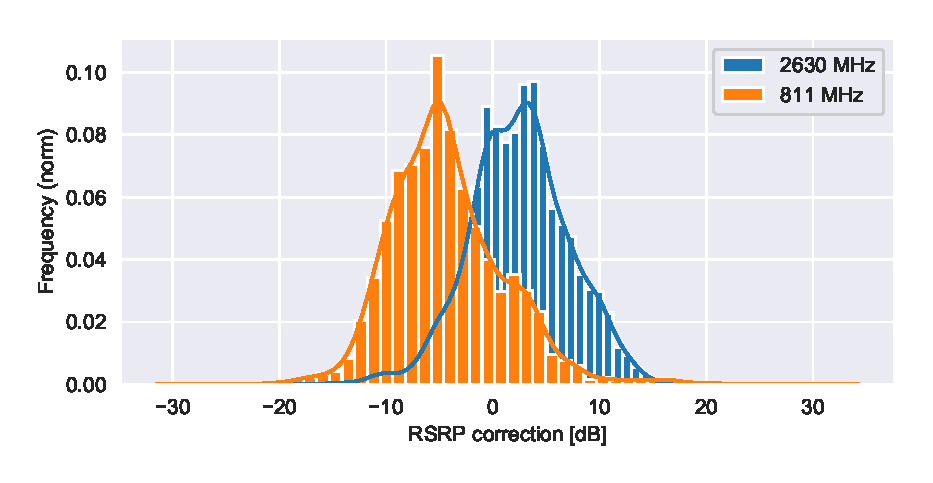
\includegraphics{chapters/part_pathloss/model_aided_paper/rsrp_correction_hist.eps}
    \caption{RSRP correction as noted by the output of $z(\cdot)$ in Eq. (\ref{eq:model}).}
    \label{fig:rsrp_correction_hist}
\end{figure}

The distributions of the \gls{rsrp} measurements and the prediction can be seen in Fig. \ref{fig:dist_pred_target} for both 811 and 2630 MHz. The performance difference between 811 and 2630 MHz, (as visualized by Fig. \ref{fig:model_comparison_bar_group}) comes to show here. A visually pleasing fit between predicted and measured is observed for 2630 MHz, while at 811 MHz, the model have issues with values of \gls{rsrp} around $-100$ to $-90$ dBm.

\begin{figure}
    \centering
    \subfloat[811 MHz]{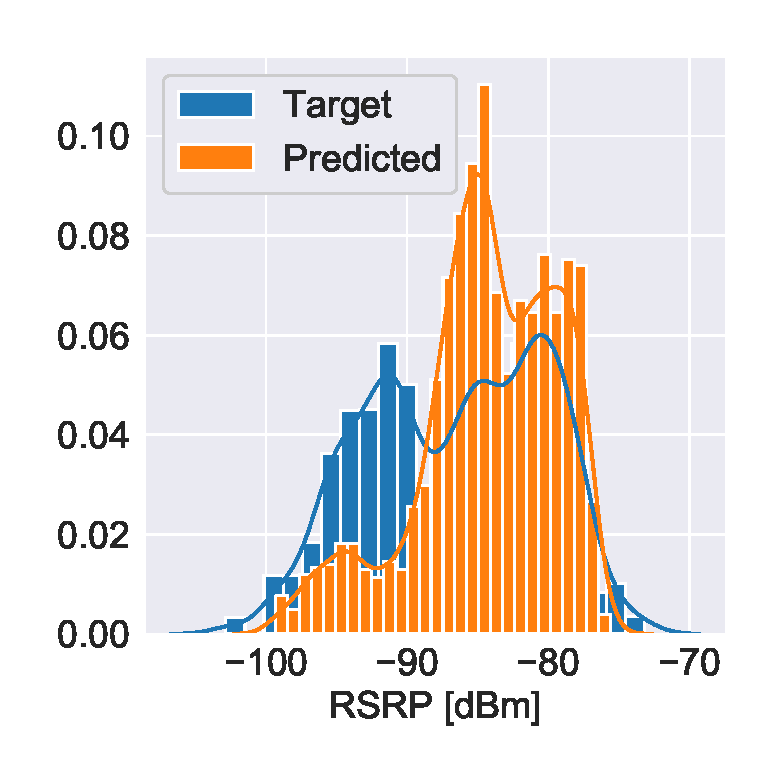
\includegraphics[width=0.4\textwidth]{chapters/part_pathloss/model_aided_paper/hist_63b17fa0-89e0-440b-952c-aa7f2e63e49c_811mhz.eps}\label{fig:dist_811}}  
    \subfloat[2630 MHz]{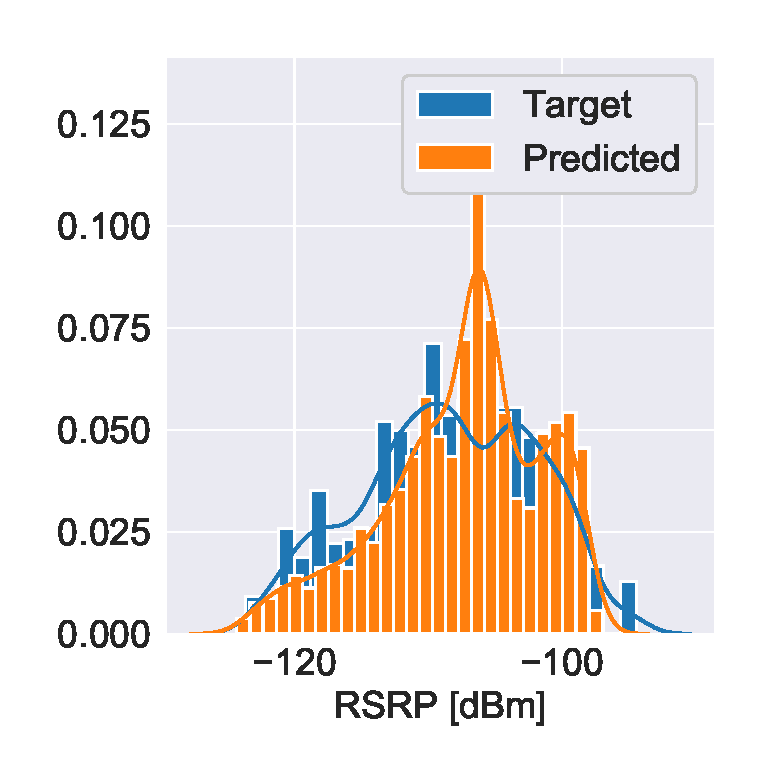
\includegraphics[width=0.4\textwidth]{chapters/part_pathloss/model_aided_paper/hist_63b17fa0-89e0-440b-952c-aa7f2e63e49c_2630mhz.eps}\label{fig:dist_2630}}
    \caption{Distribution of RSRP for 811 (a) and 2630 (b) MHz on the test set and the model output.}
    \label{fig:dist_pred_target}
\end{figure}

\subsection{Discussion}
The proposed approach is capable of outperforming traditional methods such as ray-tracing and empirical models. The predictive performance improvement at $2630$ MHz is $\approx 4.7$ dB while $\approx 1$ dB of gain is achieved at 811 MHz. The performance at 2630 MHz indicates the necessity of data describing local variability, which is not present in either the implemented ray-tracing model (limited clutter detail) or the empirical model. Clutter data is, however, observable in the proposed satellite images. The result indicates that this is not solely caused by including satellite images. The specific performance gain offered by the inclusion of the images is documented to be, on average, $\approx 0.8$ dB. Thus, the performance increase (compared to the traditional methodologies) indicate the usefulness of \gls{nn} in path loss predictions. The majority of the performance increase is not caused by the inclusion of satellite images but rather the adaptive nature of \gls{nn}. However, by including the images and aiding the model with a simple path loss model, additional improvements to performance are achieved. 

The area spanned by the image offer details of clutter, nearby buildings and even parked cars. However, the area spanned by the images might contain details not relevant to differences in frequency. For instance, higher attenuation is associated with higher frequencies when it comes to clutter data due to the lower wavelength. In this case, it might be more relevant to include a more detailed version of the image spanning a reduced area. Moreover, it might be that the images simply contain too much information necessary for relevant propagation statistics. Such insight was gained during the hyper-parameter scanning, of which many experiments were conducted. Likely, simplistic images or the vectorization of such images (e.g. footprints/outlines of buildings) may improve the predictive performance, lower the model complexity, or in any case, enhance the task of finding the best-performing hyper-parameters.

The task of hyper-parameter scanning is complex and time-consuming. From the results, it is clear that performance improvements have been achieved in both utilizing features, a simple path loss model and satellite images. However, it should be noted that the documented hyper-parameters is an attempt at an optimum solution. It is likely that better hyper-parameters can be found using extensive scanning and possibly even Machine Learning-based sampling methodologies as documented in chapter \ref{ch:mlbasics}. The model achieved requires approximately 300 experiments, each with 240 minutes of training time. The amount of experiments completed leads to the discussion of complexity. It is argued that the proposed method requires reduced complexity as compared to a traditional ray-tracing approach. The geostatistics and data necessary for local variability approximations are embedded into the supplied images and requires only the convolution and multiplication operations for extracting the \emph{correction} to a predicted path loss. It can be argued that the model only needs to be trained once, upon discovery of the best hyper-parameters. So in short, the complexity of the trained method solely lies in the prediction time and the memory necessary hereof. 

\subsection{Conclusion}\label{subsec:conclusion_v2}
The introduction of a simple path loss model (expert knowledge) for aiding the training process, in combination with satellite images, have improved the overall generalization properties of the Deep Learning model. The study items identified in \emph{version 1} have successfully been explored in an attempt to quantify the properties of the proposed approach and achieve insight into the specific prediction improvements by including satellite images. Furthermore, compare how the method performs to traditional approaches. The technique is capable of improving prediction accuracy by $\approx 1$ dB at $811$ MHz and $4.7$ dB at $2630$ MHz. The model provides an average prediction error of $\approx 4.1$ dB when predicting \gls{rsrp} in an unseen area for both $811$ and $2630$ MHz, which is a significant improvement to traditional methodologies. It is furthermore concluded that the complexity of the model is primarily associated with the untrained model, e.g. hyper-parameters and the selection hereof. The trained model is capable, with only position and available satellite images to produce an accurate prediction of received power in unseen areas.
